\cleartooddpage[\thispagestyle{empty}]
\chapter{The Dark Matter Paradigm}\label{ch_dm}

  Dark matter makes up 26.5\% of the universe's energy and 81.5\% of its mass~\cite{planck2015}.
  It has had a significant impact on the development of the universe, shaping its present day distribution.
  This chapter discusses the main features of dark matter physics.
  These include the astrophysical evidence for the existance of dark matter, an outline of the current cosmological paradigm of $\Lambda$CDM and the Standard Model, as well as arguments for why dark matter may be in the form of a new, unknown particle.

  %From: https://arxiv.org/abs/1502.01589 , Table 3, column [4] :
  %  omega_b h^2 = 0.02225
  %  omega_c h^2 = 0.1198
  %  H_0         = 67.27 km / s / Mpc
  %  h           = H_0 / ( 100 km / s / Mpc ) = 0.6727
  %thus:
  %  omega_b = 0.02225 / h^2 = 0.0491 =  4.9% of universe's energy is in baryonic matter
  %  omega_c = 0.1198  / h^2 = 0.2647 = 26.5% of universe's energy is in dark matter
  %  ( 26.5 - 4.9 ) / 26.5 = 81.5% of universe's mass is stored in dark matter

\section{Astrophysical Evidence for Dark Matter}
  
  The current effects attributed to dark matter can be grouped into three observable physical effects, and four different length scales.
  These physical effects include observations of gravity pulling on electromagnetic emitters, gravity bending background light, and the universe's total energy budget.
  On the smallest length scales, concentrations of several thousand stars can be seen revolving around their center of mass, at a larger distribution of speeds than one would expect from the existing visible amount of matter.
  At larger scales the optical light from galaxies, as well as hydrogen lines, can be used to measure the amount of mass and its rotational velocity around the center of galaxies.
  At even larger scales, galaxy velocities can be measured and compared, X-ray telescopes can monitor the amount of hot gas, and mass-heavy areas of space will gravitationally lens background galaxies.
  At the the largest scale, the measurement of oscillations in the cosmic microwave background can be used to determine the amount of dark and baryonic matter.
  
  \subsection{Scales of $10^{19}\:\text{m}$ : Dwarf Galaxies}\label{dm_dwarfscale}
    % 10^19m comes from: 
    % fornax dwarf spheroidal galaxy wiki page
    %    17' x 12.6' in solid angle, call it 15'
    %    140kpc away  
    %    140kpc * Tan(15') = 0.6kpc = 1.8*10^19m ~ 10^19m
    At scales of $\nicetilde 10^{19}$m, groups of thousands stars, called satellite galaxies or dwarf galaxies, lie at the edge of full size galaxies like our own.
    These dwarf galaxies are strong evidence for dark matter because their luminous matter is not enough to gravitationally bind them.
    An example of a dwarf galaxy is shown in Figure~\ref{fig:sculptor}, the Sculptor dwarf galaxy, imaged in the optical frequencies by the MPG/ESO Telescope.

    \begin{figure}[h]
      \centering
      \includegraphics[width=0.95\textwidth]{images/sculptor/sculptor.eps}
      \caption[Sculptor Dwarf Galaxy]{
        The Sculptor Dwarf Galaxy~\cite{sculptor_image}, imaged with the MPG/ESO telescope~\cite{sculptor_paper}.
        This dwarf galaxy has a $\frac{M_\odot}{L_\odot}$ ratio of 15.3~\cite{sculptor_ml}.
      }
      \label{fig:sculptor}
    \end{figure}

    Measuring the mass of these dwarf galaxies is done in two ways.
    In the first, telescopes observed the individual spectra of these stars, allowing for their line-of-sight velocity to be calculated~\cite{dwarf_gal_red_giant}.
    The width of the distribution of the velocities is called the velocity dispersion.
    By looking at this velocity dispersion, the total mass of the dwarf galaxy can be inferred~\cite{dwarf_gal_vel_dispersion, dwarf_gal_vel_dispersion2}.
    What makes this possible is that the velocity dispersion of a group of stars is proportional to the total mass of the graviational well.
    This can be seen by applying the virial theorem.
    The virial theorem, Equation~\ref{eqn:virial}, states an n-body system in equilibrium will always have the same ratio of kinetic energy $T$ to potential energy $V$, as long as the gravitational potential is proportional to $r^-1$.

    \begin{equation}\label{eqn:virial}
      T = \frac{V}{2}
    \end{equation}

    The kinetic energy of a group of massive objects is Equation~\ref{eqn:kineticen}.
    
    \begin{equation}\label{eqn:kineticen}
      T = \sum_i \frac{1}{2} m_i \left \langle v_i^2 \right \rangle = \frac{1}{2} M \left \langle v^2 \right \rangle
    \end{equation}
    
    Where $m_i$ is the mass of each star, $v_i$ is the velocity of each star, $M$ is the total mass of all stars.
    The same can be done with galaxies within a cluster as well, instead of stars within a galaxy.
    The total potential energy is Equation~\ref{eqn:potentialen}.

    \begin{equation}\label{eqn:potentialen}
      V = ??
    \end{equation}
    % see: http://www.jb.man.ac.uk/~gp/PHYS_30392/12_CSM13_Density_of_the_Universe_II_b.pdf
    
    % from : http://iopscience.iop.org/article/10.1086/518357/pdf
    %   eqn 1: M = 10 r_hp \sigma^2_r / G
    %     r_hp : half light radius
    %     \sigma_r : 1D line-of-sight velocity dispersion
    %     G : newtons gravitational constant
    %     from Spitzer 1987
    
    % from : http://iopscience.iop.org/article/10.1086/521998/pdf
    %   nfw halo from velocity dispersion calculated from eqn [A15] of Mamon & Lokas 2005
    
    When Equations~\ref{eqn:virial}, \ref{eqn:kineticen}, and \ref{eqn:potentialen} are combined, $M$ can be solved for, only as a function of the velocities{\color{red}(??)}.
    \begin{equation}\label{eqn:virial_combined}
      \frac{1}{2} M \left \langle v^2 \right \rangle = \frac{1}{2} ??
    \end{equation}
    
    Thus, by measuring stellar velocities and calculating the total kinetic energy of a group of stars, the potential energy can be calculated, which indicates the amount of mass present in the group.
    As stellar velocity measurements rely on doppler-shifted spectral lines, and not the star's absolute brightness, any derived mass estimates are fairly resistant to changes in observed brightness.
    These changes in brightness can be from atmospheric variations during telescope observations or changes in the amount of light-absorbing dust in the line-of-sight.

    The second way to measure galaxy masses is by measuring the total brightness of a galaxy, and divide by the luminosity of the Sun $L_\odot$.
    This then indicates the number of solar masses $M_\odot$ contained in the galaxy, a measure of its baryonic (i.e. 'bright', not dark) mass.
    For these conversions, nominal values are $M_\odot =$ \SI{1.9885e30}{kg} and $L_\odot =$ \SI{3.828e26}{W}, though different authors may use slightly different values depending on the year of publication~\cite{iau_solarconstants}.
    % from https://arxiv.org/pdf/1510.07674.pdf
    % L_\odot from page 3, table "SOLAR CONVERSION CONSTANTS" 
    % M_\odot :
    %   G*M_\odot = 1.3271244e20 m^3 s^-2 (from table "SOLAR CONVERSION CONSTANTS")
    %   G = 6.67408e-11 m^3 kg^-1 s^-2
    %   thus 
    %   M_\odot = 1.3271244e20 m^3 s^-2 / 6.67408e-11 m^3 kg^-1 s^2
    %           = 1.98847e30 kg
    
    The first way measures the 'total' mass from the rotational profile, while the second only measures the mass of its 'luminous' parts.
    The ratio of the 'total' mass divided by the 'luminous' mass is called the mass-to-light ratio, which indicates the amount of dark matter present in the galaxy~\cite{faber_ml}.
    Dwarf galaxies have mass-to-light ratios of around 5-100 $\frac{M_\odot}{L_\odot}$, but can reach up to \nicetilde 1000~\cite{Simon2007_dwarfgalaxykeck}.
    These high values are considered strong evidence in favor of dark matter.
    A random assortment of Local Group dwarf galaxies and their $\frac{M_\odot}{L_\odot}$ is shown in Table~\ref{tab:mlratios:dwarfgals}.
    
    \begin{table}[]
      \centering
      \caption[Ratios of $\frac{M_\odot}{L_\odot}$ for Various Dwarf Galaxy Objects]{Ratios of $\frac{M_\odot}{L_\odot}$ for various dwarf galaxy objects~\cite{localdwarfs}.}
      \label{tab:mlratios:dwarfgals}
      \begin{tabular}{l r}
        Object      &  Mass, $\left [ \frac{M_\odot}{L_\odot} \right ]$ \\
        \hline
        IC 10       &  0.1 \\
        NGC 147     &  7.1 \\
        NGC 185     &  2.5 \\
        NGC 205     & 12   \\
        LGS 3       & 21   \\
        IC 1613     &  1.4 \\
        Carina      & 30   \\
        Antlia      &  7.4 \\
        Leo I       &  3.1 \\
        Sextans     & 34   \\
        Ursa Minor  & 60   \\
        Draco       & 58   \\
        Sagittarius & 22   \\
      \end{tabular}
    \end{table}
    
    As an additional piece of evidence for dark matter, dwarf galaxies near the Perseus cluster were studied.
    From the gravitational potential of their baryonic mass alone, these dwarf galaxies should be ripped apart by the tidal disruption of the Perseus cluster.
    Instead, observations of these dwarf galaxies indicate they remain intact, leading to the conclusion that the presence of dark matter is providing extra gravitational force~\cite{Penny2009}.
    
    \FloatBarrier

  \subsection{Scales of $10^{20}\:\text{m}$ : Galaxies}\label{dm_gal}
    %
    % galaxy rotation curve wiki page, M33 has curve measurements out to 50,000ly
    %   50,000ly = 4.7*10^20m ~ 10^20m
    At scales of $\nicetilde 10^{20}$m, the effects of dark matter on galaxies are observable.
    Within galaxies, the amount of light observed in a sector predicts a lower amount of mass, while observing the line-of-sight velocity predicts a higher amount of mass.
    
    In the first prediction technique, the total amount of light produced by a quadrant of a galaxy is measured with optical telescopes.
    Then, as in Section~\ref{dm_dwarfscale}, the amount of light produced can be compared with the Sun as a standard mass-to-light ratio, allowing for a prediction of the amount of mass contained in that sector.
    Known mass-to-light ratios can then be used to calculate the total amount of mass within that quadrant.
    For example, in a survey of 25 galaxies in Ref. \cite{galaxy_mass_light_ratio}, most possesed a mass-to-light ratio of 1 to 10.

    In the second prediction technique, a galaxy's emission spectrum is observed at many positions around its disk (center, outer edges, etc).
    By comparing the orientation of the disk with the doppler-shifted position of well-known spectral lines, one can calculate the average velocity that each section is traveling at around the center of its galaxy, forming a rotation curve~\cite{rotation_curve_review, spiral_galaxy_rot_curve, milkyway_dm_evidence}.
    Newton's law of gravity can then be used to calculate the mass contained within a sphere of that same radius.
    This calculation results in a larger amount of mass than the one found simply from the total amount of light observed.
    
    In Figure~\ref{fig:m33rotcurve}, a rotation curve from M33 observations is shown.
    The observed velocity curve (the datapoints) continues to increase at larger radii.
    If the galaxy was only made of stars, then the rotation curve would follow the short dashed line.
    If the galaxy was only made of gas, then the rotation curve would instead follow the long dashed line.
    As these two major components do not combine to form the observed rotation curve, the presence of dark matter can account for the difference, shown as the dashed-dotted line~\cite{m33rotcurve}.
    
    \begin{figure}[ht]
      \includegraphics[width=0.9\textwidth]{images/m33rotcurve/m33rotcurve.eps}
      \caption[M33 Rotation Curve]{
        The rotation curve from M33~\cite{m33rotcurve}.
        The solid line is the best fitting model to the observed velocity measurments.
        The short dashed line is the stellar disk contribution, the gas contribution is the long dashed line, and the dashed-dotted line is the dark matter contribution.
      }
      \label{fig:m33rotcurve}
    \end{figure}
    
    \begin{table}[]
      \centering
      \caption[Ratios of $\frac{M_\odot}{L_\odot}$ for Various Galactic-scale Objects]{Ratios of $\frac{M_\odot}{L_\odot}$ for various galactic-scale objects~\cite{faber_ml}.}
      \label{tab:mlratios}
      \begin{tabular}{l r}
        Object      &  Mass, $\left [ \frac{M_\odot}{L_\odot} \right ]$ \\
        \hline
        M31 (Andromeda) &  7.6  \\
        M33             &  4.5  \\
        M51             &  3.3  \\
        M81             &  8.5  \\
        NGC 801         &  2.4  \\
        NGC 2403        &  5.5  \\
        NGC 2841        & 10.6  \\
        NGC 4324        &  5.5  \\
        NGC 6822        &  0.58 \\
      \end{tabular}
    \end{table}
      
    A random sample of galaxies from Ref. \cite{faber_ml} are shown alongside their mass-to-light ratios in Table \ref{tab:mlratios}.
    Our own Milky Way galaxy is measured to have a mass to light ratio of \SIrange{1.2}{1.5} $\frac{M_{\odot}}{L_{\odot}}$~\cite{milkyway_ml_ratio}, indicating for every 5 sun-like stars in our galaxy, there are another two stars worth of dark matter.
    
    The further evidence of dark matter can also be deduced through additional weak gravitational lensing~\cite{weak_lensing_2001}.
    Lensing elliptical galaxies can constrain mass profiles, as the amount of lensing indicates the total amount of mass, which in turn limits the amount of dark matter present at different radii~\cite{weak_lensing_ellipse}.

    \begin{figure}
      \centering
      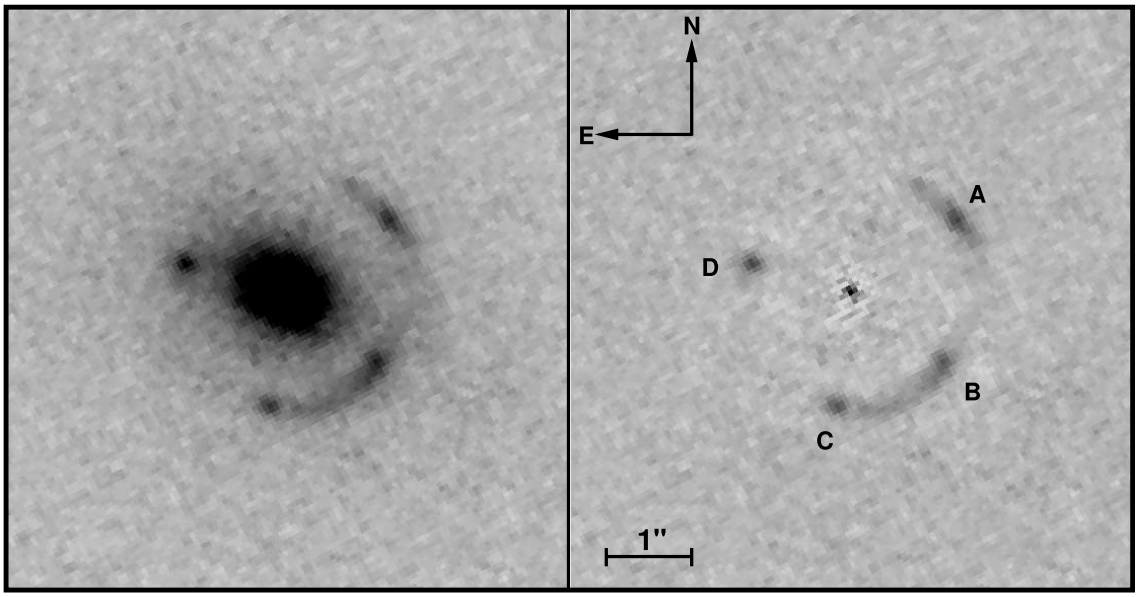
\includegraphics[width=0.95\textwidth]{images/weak_lensing_ellipse/weak_lensing.pdf}
      \caption[Weak Lensing with an Ellipse Galaxy]{
        Galaxy 0047-281 imaged by the Hubble Space Telescope, from Ref. \cite{weak_lensing_ellipse}.
        Left: Original image.
        Right: Same as Left but with the central foreground galaxy subtracted, leaving behind 4 lensed images A, B, C, and D of a background galaxy.
      }
      \label{fig:ellipse}
    \end{figure}
    
    
    Galaxy lensing can be used to estimate the size of the substructure of a lensing galaxy, based on the 4 lensed images of a quasar~\cite{weak_lensing_quasar}.
    The spectra of the four lensed images vary in brightness and distortion.
    These variations can be seen by looking at the ratio of the widths of different spectral lines.
    These ratios of different lensed images indicate that there exists variations in the mass density in the lensing galaxy.
    These variations are best fit by randomly distributing spheres of lensing mass throughout the lensing galaxy, each having a mass of \SI{10^6}{\Msol}.
    This spheres of this mass are consistant with the scale of dark matter substructure predicted by CDM.


  \subsection{Scales of $10^{23}\:\text{m}$ : Galaxy Clusters}\label{dm_galclusters}
    %
    % galaxy cluster wiki page
    % 2-10 Mpc, call it 6Mpc = 1.85*10^23m ~ 10^23m
    At scales of $\nicetilde 10^{23}$m, dark matter's effects on galactic clusters become observable with several techniques.
    In one technique, the mass-to-light ratio can be measured for galaxy clusters.
    This is done the same as with dwarf galaxies; luminous mass is derived from the brightness of the cluster, while total mass is measured from the velocity dispersion of individual galaxies within the cluster.
    From measurements of several hundred galaxy clusters, it was found that galaxy clusters have mass-to-light ratios of \SIrange{10}{1000}{$\frac{\Msol{}}{\Lsol{}}$}~\cite{cluster_ml_ratios}, indicating a very high amount of dark matter is present in these objects.

    \begin{table}
      \centering
      \caption[Ratios of \MLsol for Various Galaxy Clusters]{Ratios of \MLsol for various galaxy clusters~\cite{cluster_ml_ratios}.}
      \label{tab:cluster_ml_ratios}
      \begin{tabular}{l r}
        Object      &  Mass, \MLsol \\
        \hline
        Abell 85   & 445 \\
        Abell 458  & 401 \\
        Abell 999  & 100 \\
        Abell 1228 & 37  \\
        Abell 2426 & 80  \\
        Abell 3122 & 960 \\
        Abell 3126 & 491 \\
        Abell 3354 & 94  \\
        Abell 3695 & 180 \\
        Abell 3921 & 175 \\
      \end{tabular}
    \end{table}
    
    Another technique for measuring the total mass is by examining the amount of gravitational lensing caused by a cluster.
    When a massive galaxy cluster has a galaxy directly behind it, the image of the background galaxy gets distorted.
    The shape of the distorted image can then be used to infer the amount of total mass in the galaxy cluster.
    Then comparing this total mass to the luminous mass provides an estimate for the amount of dark matter contained in the galaxy cluster.
    This was used with galaxy clusters Abell 370 and CL 2244-02 to estimate the amount of dark matter in each~\cite{cluster_lensing}.
    Lensing cluster Abell 370 and several distorted background galaxies are shown in Figure~\ref{fig:abell370}.
    This technique found that for both Abell 370 and CL 2244-02, a large amount of dark matter is required to fit the observed arcs, within the range of 200-1000 \MLsol.
    
    \begin{figure}
      \centering
      \includegraphics[width=0.95\textwidth]{images/abell370/abell370_cropped.pdf}
      \caption[Gravitational Lensing in Abell 370]{
        Galaxy cluster Abell 370 is shown here, along with many gravitationally lensed background galaxies.
        The large arc marked by the green lines is the distorted background galaxy image used to calculate the cluster's total mass~\cite{cluster_lensing}.
        Credit: NASA, ESA/Hubble, HST Frontier Fields~\cite{abell370_hubble}.
      }
      \label{fig:abell370}
    \end{figure}
    
    Another example of using gravitational lensing to measure dark matter mass is with cluster Cl0024+1654.
    This galaxy cluster creates several lensed images of the same background galaxy, which are used to measure the total mass
    The lensing is shown in Figure~\ref{fig:stronglens}, where the blue arcs are the distorted background galaxy images.
    From all of these lensed images, the best fit amount of dark matter indicates this cluster has a mass-to-light ratio of \SI{230}$\,h_{70}\,$\MLsol, where $h_{70}$ is set to $0.70$~\cite{cluster_strong_lensing_1996, cluster_strong_lensing_1998, cluster_strong_lensing_2010}.
    
    \begin{figure}
      \centering
      \includegraphics[width=0.95\textwidth]{images/cluster_strong_lensing_8/stronglensing2.pdf}
      \caption[Gravitational Lensing in Cl0024+1654]{
        Strong lensing of a blue background galaxy by galaxy cluster Cl0024+1654 into multiple blue distorted images~\cite{cluster_strong_lensing_1996}.
      }
      \label{fig:stronglens}
    \end{figure}
    
    Yet another way of measuring the total mass of a cluster is by examining X-ray measurements.
    In galaxy clusters, the majority of the luminous mass is stored in warm ($kT\simeq\,$\SI{5}{keV}) gas, rather than stars.
    This warm gas emits X-rays, which can be detected by satellites like Chandra~\cite{chandra}.
    By measuring the X-ray flux at the center of the galaxy cluster Abell 2029, the total mass of the cluster can be measured.
    This is done by assuming the warm gas is in hydrostatic equilibrium, where the force of gravity towards the cluster center is equally balanced by the pressure of the warm gas.
    This implies that when moving outwards from the cluster center, the density and temperature of the gas is predictable.
    From this, the mass-to-light ratio can be inferred at several different radii from the cluster center.
    Within \SI{20}{$\,h_{70}^{-1}$ kpc} of the center, the ratio is 12 \MLsol, while beyond a radius of \SI{200}{$\,h_{70}^{-1}$ kpc} the ratio rises above 100 \MLsol{}, indicating a high amount of dark matter is present~\cite{cluster_chandra}.
    {\color{red}(Here we reference 200 $h_{70}^{-1}$ kpc, but in the previous paragraph we reference 230 $h_{70}$, is this consistant? ask orel??)}
    
    These previously mentioned techniques have been combined into an analysis of galaxy cluster 1E 0657-558 to provide a cardinal piece of evidence in favor of particle dark matter.
    Galaxy cluster 1E 0657-558 consists of two subgroups of galaxies, a larger 'target' cluster, and a smaller Bullet cluster.
    Each cluster's mass is contained in two clouds; gas and stars that form the baryonic cloud, and the much more massive dark matter cloud.
    The baryonic cloud is visible through Chandra X-ray observations, which is able to image the warm ($kT\simeq\,$\SI{10}{keV}) gas and infer its density.
    The dark matter cloud is inferred through weak lensing observations, where the mass of the cluster distorts the images of background galaxies.
    In this pair of clusters, the Bullet cluster has fallen through the target cluster.
    However, the two clouds of the Bullet cluster dragged on the clouds of the target cluster, and dragged at different rates.
    This difference in drag over time resulted in a separation between the Bullet cluster's baryonic and dark matter clouds.
    , visible in Figure~\ref{fig:bullet}.

    \begin{figure}[ht]
      \centering
      \includegraphics[width=0.95\textwidth]{images/bulletcluster/bulletcluster_cropped.pdf}
      \caption[The Bullet Cluster]{
        The Bullet Cluster~\cite{bullet_cluster_combined_image}.
        The blue clouds indicate the graviational lensing mass~\cite{bullet_cluster}, the pink represents clouds of warm gas emitting X-rays~\cite{bullet_cluster_chandramap}.
        The red triangle indicates the bullet cluster's warm gas center-of-mass, and the blue oval marks the approximate center of the weak lensing (dark) mass.
        The remaining stars and galaxies are imaged in the optical spectrum~\cite{bullet_cluster_composite}.}
      \label{fig:bullet}
    \end{figure}
    
    The pink clouds are X-ray observations of the cluster's warm gas, while the blue clouds are the weak lensing mass.
    The red triangle and blue oval show the approximate centers of mass of the bullet cluster's two clouds.
    The difference in position between the two centers of mass allows for constraints to be put contraints on the mass and cross section.
    This contraint is shown in Equation~\ref{eqn:bullet}, where $\sigma_{\chi}$ is the dark matter particle cross section, and $m_{\chi}$ is the dark matter particle mass~\cite{bullet_cluster,bullet_cluster2}.
    
    \begin{equation}\label{eqn:bullet}
      \frac{\sigma_{\chi}}{m_{\chi}} < 1 \, \textrm{cm}^2 \, \textrm{g}^{-1}
    \end{equation}
    
    This result was improved by combining 72 galaxy cluster collisions, improving the limit in Equation~\ref{eqn:bullet} to \SI{0.47}{$cm^{2} g^{-1}$}~\cite{cluster_72}.


  \subsection{Scales of $10^{26}\:\text{m}$ : The Observable Universe}\label{dm_universe}
    %\subsection{Inter-Cluster Scale}
    % age of universe (13.82*10^9 years * speed of light) = 1.307*10^26m
    At the universe's largest scale, $\nicetilde 10^{26}$m, the Cosmic Microwave Background (CMB) has been used to measure the total amount of dark matter in the universe.
    By looking at the structure of the CMB, the structure of the universe and its particle populations can be studied, including how they developed and changed from the big bang to the present day.
    In order to understand dark matter's place in the evolution of the universe, several important moments must be discussed.
    The first moment of the universe was Inflation, where a singularity with a temperature of $kT=10^{17}\:\textrm{GeV}$ quickly expanded as a quark-gluon plasma and cooled~\cite{inflation0,inflation1,inflation2,inflation3}.
    Once the average temperature had reduced enough, quarks could bind together to form baryons, in a stage known as Baryogenesis.
    The time/temperature that Baryogenesis occurred at has not been determined.
    However, there are several competing theories that may explain how an unequal ratio of baryons to antibaryons were created~\cite{baryogenesis1,baryogenesis2}.
    
    At this point, the universe is a sea of photons, electrons, and baryons.
    Once the universe cooled below the electron-proton binding energy, electrons were captured by protons in great numbers.
    These captured electrons then release photons as they relaxed to the ground state.
    Since electrons and protons have formed electrically neutral hydrogen atoms, the universe is transparent to these photons, which are free to travel the universe~\cite{planck2015,theEarlyUniverse,CMBFundamentals,CMBFlat}.
    These blackbody photons are called the cosmic micrwave background.
    Since these are photons emitted by the last electrically charged particles, density variations in the charged particles produce density variations in the cosmic microwave background.
    Studying the spectrum of these density variations allows for models of the big bang theory and of the universe's development to be tested.
    
    During this time, a background population of WIMP dark matter particles were repeadtedly created and annihilated.
    After the universe expanded further, the density of these WIMPs decreased to the point where they were no longer running into each other.
    This increased WIMP transparency froze the number of WIMPs at that time, called the relic density.
    From the equation (??).
    
    % see http://pdg.lbl.gov/2013/reviews/rpp2013-rev-dark-matter.pdf for more basic info
    % see https://arxiv.org/pdf/1603.03797.pdf
    
    After that freezout, the temperature was low enough that baryon creation and annihilation rates plummited.
    Thus, the number of baryons that were in the universe at the freezout temperature determines how many baryons are in existance today, since there are no significant ways to destroy universe-scale quantities of baryons.
    This freezout left an imprint of its structure, where higher and lower densities of remaining baryons led to higher and lower densities of CMB photons.
    {\color{red}(This is not entirely accurate (the fraction of baryons to anti-baryons is too high to be explained as a simple statistical fluctuation which froze).
Also, it does not really explain how dark matter plays a role (you mention it in the next paragraph, but it is not explained). -Orel ?? )}
    

    From this structure, the composition of the universe can be modeled.
    In terms of energy, 68.6\% of the universe is stored in Dark Energy, a repulsive force which causes almost all visible galaxies to accelerate away from the Milky Way.
    % 100% - ( 26.5% + 4.9 ) = 73.5% (from beginning of chapter)
    Another 4.9\% of the universe's energy is stored in baryonic matter, like protons and neutrons.
    The remaining 26.5\% of the universe's energy is contained in dark matter~\cite{planck2015}.

    Another important piece of evidence for the existance of dark matter is the abundance of Deuterium present in the universe.
    The amount of Deuterium that was left over from the big bang depends on the amount of baryons in the universe.
    The amount of baryons predicted by this is not enough to account for the total mass of the universe, thus it must exist in other (darker) particles.
    {\color{red}(The abundance of Deuterium is relevant for the argument of baryonic/non-baryonic dark matter. Meaning, it does not directly point to the existence of dark matter, but more suggests about its nature. It is a good point to bring up (and expand), but probably in a different section, no? -Orel ??)}
    Most theories of dark matter being trapped in cold dead stars, referred to as MAssivly Compact Halo Objects (MACHOs), have been abandoned due to this baryon limitation {\color{red}(cite??)}.

    Another measurement that depends heavily on the presence of dark matter is the rate at which galaxies form clumps.
    In the Sloan Digital Sky Survey (SDSS), the positions of 1.6 million galaxies, quasars, and stars are mapped~\cite{sdss_release}.
    By simulating the distribution of similar objects as the universe ages, only with a dark matter component does the universe form clumps that match SDSS observations.
  
    {\color{red}(Take a few more ideas from the primer \cite{DMPrimer}, explain them, then leave out the above line altogether (??))}

    {\color{red}(baryon acoustic oscillations?? \url{http://iopscience.iop.org/article/10.1086/466512/meta} )}
    
    {\color{red}(cmb temperature and polarization??)}
    
    % borrow dark matter-related events from this chart?
    % https://en.wikipedia.org/wiki/Chronology_of_the_universe
    %\begin{table}[h]
    %  \centering
    %  \caption[Key Events During the Life of the Universe]{
    %    Key events during the development of the universe.
    %    The Time column is the age of the universe at that event.
    %    The Temperature column is the universe's average temperature at that time.
    %    The Distance column is how far light could have traveled in that time, if it started at the beginning of the universe and travelled at present-day $c$.
    %    {\color{red}Idea from \url{http://www.th.physik.uni-bonn.de/drees/non\_ac/presentation\_Narimani.pdf} , slide 10, CREDIT THIS!!}
    %    {\color{red}(Source remaining values??)}
    %    {\color{red}(If a term is mentioned here, it needs to be explained!! ??)}
        % see http://www.sciencedirect.com/science/article/pii/S0370157304003515 page 286 for more info
        % see https://arxiv.org/pdf/hep-ph/0602002.pdf
        % maybe check PDG?
        % http://www.particleadventure.org/history-universe.html
    %  }
      % Space column is just Time column * 3e8 m/s
    %  \label{cosmo_events}
    %  \begin{tabular}{lcc}
    %    Event                                         & Time                    & Temperature                \\
    %    \hline
    %    Big Bang (Planck Time \& Temp)                & $10^{-43}\,$s           & $10^{19}\,$\GeV            \\
        % https://www.physics.umd.edu/courses/Phys741/xji/chapter2.pdf , pg 22, equation 2.10/2.11
        % planck mass
        % M_{pl} = \sqrt{ \frac{ \hbar c }{ G_N } } = 1.22*10^19 GeV
        % hbar : reduced planck constant
        % c    : speed of light
        % G_N  : newtons gravitational constant
        % planck time t_P = ~10^-43 s

    %    Inflation                                     & $10^{-34}\,$s (?)       & ??                         \\
    %    Baryogenesis                                  & ??                      & ??                         \\
    %    ElectroWeak phase transition                  & \SI{20}{ps}             & \SI{100}{\GeV}             \\
    %    Dark Matter Freeze-out                        & ??                      & ??                         \\
    %    QCD phase transition                          & \SI{20}{\mu.s}          & \SI{150}{\MeV}             \\
    %    Neutrino decoupling                           & \SI{1}{s}               & \SI{1}{\MeV}               \\
    %    Neutron freezout                              & \SI{1}{s}               & \SI{1}{\MeV}               \\
    %    $\text{e}^+ - \text{e}^-$ annihilation        & \SI{6}{s}               & \SI{500}{keV}              \\
    %    Big Bang nucleosynthesis                      & \SI{3}{min}             & \SI{100}{keV}              \\
    %    Matter and radiation densities equal          & \SI{60}{kyr}            & \SI{0.75}{eV}              \\
    %    (ion?) Recombination                          & \SIrange{260}{380}{kyr} & \SIrange{0.26}{0.33}{eV}   \\
    %    Photon decoupling                             & \SI{380}{kyr}           & \SIrange{0.23}{0.38}{eV}   \\
    %    Reionization                                  & \SIrange{100}{400}{Myr} & \SIrange{2.6 }{7   }{meV}  \\
    %    Dark energy-matter equality                   & \SI{9}{Gyr}             & \SI{0.33}{meV}             \\
    %    Present                                       & \SI{13.8}{Gyr}          & \SI{0.24}{meV}             \\
    %  \end{tabular}
    %\end{table}
    

\section{$\Lambda$CDM Cosmology and the Standard Model}

  At the largest spatial scales, $\Lambda$CDM is the currently accepted model of cosmology.
  The $\Lambda$ refers to the density of dark energy, while CDM refers to Cold Dark Matter.
  $\Lambda$CDM models how the universe expanded from the big bang until the present day universe.
  This model predicts the different times particles froze out of the universe, and their resulting distributions.

  A large part of $\Lambda$CDM comes from measuring fluctuations in the Cosmic Microwave Background (CMB).
  In these fluctuations, a snapshot of the universe when it was 380,000 years old is preserved, providing many clues as to the development of the universe, including its age, energy content, structure, and expansion. 
  {\color{red}(You should explain what is learned from the CMB and how. -Orel ??)}
  This CMB snapshot also provides hints about the nature of dark matter, including some basic requirements for any potential dark matter candidate particle.

  \begin{figure}[ht]
    \includegraphics[width=0.95\textwidth]{images/cmb_skymap/cmb_skymap.eps}
    \caption[The Cosmic Microwave Background]{
      The cosmic microwave background temperature map of the universe \cite{wmap_skymap}, from 9 years of WMAP observations~\cite{wmap9year}.
      This image shows a temperature range of \SI{\pm200}{\mu{}Kelvin}.
    }
    \label{fig:cmb}
  \end{figure}

  The current paradigm of particle physics is called the Standard Model~\cite{standardmodel}.
  It consists of groups of particles called quarks and leptons, as well as the bosons that mediate interactions between these particles.
  Quarks combine to form hadrons, like protons and neutrons, and mesons, while leptons consist of electrons, muons, tauons, and their neutrino companions.

  At the forefront of dark matter search candidates are particles predicted by Supersymmetry~\cite{Jungman:1995df}, (specifically Minimal Supersymmetric Standard Model, or MSSM~\cite{MSSM,supersym1}), an extension to the Standard model.
  Much like how all particles have an anti-particle, in supersymmetry, each Standard Model quark, lepton, and boson, has a supersymmetric partner particle.
  Quarks and leptons have squarks and sleptons as their supersymmetric partners, while bosons have partners like photinos, gluinos, and charginos.
  While no evidence of supersymmetry has been discovered to date, it is still preferred due to its ability to predict physics across a large range energy scales, the holy grail of any Grand Unified Theory.
  

\section{Particle Dark Matter}\label{sec_particledm}

  Since none of the Standard Model particles meet the conditions to be a dark matter candidate, theoretically predicted particles are now the focus of most searches.
  One recently favored Standard Model dark matter candidate was the neutrino, due to its numerous nature and lack of interaction with the strong and electromagnetic forces.
  This was generally referred to as Hot Dark Matter, as neutrinos travel at relativistic speeds.
  However, it was eventually demonstrated that because of these relativistic speeds, neutrinos would diffuse out of their initial overdensities.
  This would result in large super-cluster-scale gravitational wells forming first, then cluster-scale wells, then galaxy-scale wells, called top-down structure formation.
  When observations are made of earlier times, the opposite is found: galaxy-scale gravitational wells form first, then cluster-scale wells, then super-cluster-scale wells in present times, called bottom-up formation.
  As this is the opposite of what is expected for relativistic dark matter, neutrinos were ruled out as a dark matter candidate~\cite{neutrinoHeirarchical}.
  % from this discussion: https://physics.stackexchange.com/questions/158319/why-are-neutrinos-ruled-out-as-a-major-or-even-sole-component-of-dark-matter
  In addition, limits on the mass of the neutrino ($\sum{}m_{\nu} = 0.194 \; \textrm{eV}, \; 95\% \; \textrm{C.L.}$) also rule it out since they are not numerous enough~\cite{planck2015}.
  % see table 5, sum m_nu [eV] row, TT, TE, EE+lensing+ext column
  
  
  Any dark matter candidate particle that meets the cosomological and particle conditions is called a WIMP, or Weakly Interacting Massive Particle.
  The currently favored WIMP candidate is the neutralino, the lightest supersymmetric particle~\cite{neutralino1}.
  {\color{red}(why neutralino??, what are its properties?)}
  One of the major predictions from particle physics and cosmology is referred to as the "WIMP Miracle".
  In it, particle physics and cosmology separately predict that if dark matter is WIMP, it should have a velocity-averaged cross section of around \SI{ 3e-26 }{ cm$ {}^3 $s$ {}^{-1} $ }, though each field comes to this value by very separate math. {\color{red}(cite??)}
  {\color{red}(It's not exactly math, there is some physical constraints in it. Can you find a better way of explaining it?? -Orel)}

  Supersymmetry predicts the existance of a WIMP-like particle with a cross section of around \nicetilde{} \SI{3e-26}{ cm${}^2$ }~\cite{Jungman:1995df}.
  % $3*{10}^{-26}\ {\textrm{cm}}^{2}$
  What made this WIMP particle a more promising candidate is that several cosmological problems can also be solved by a weakly-interacting GeV-TeV mass particle.
  {\color{red}What were these cosmological problems that were fixed??}
  Thus, two separate fields of physics recognized that they both were looking for a WIMP-like particle within the same mass and cross section range.

  In $\Delta$CDM cosmology, the relic density is all of the leftover dark matter particles after the universe became too cold to produce more dark matter particles.

  {\color{red}One or two more sentences on the relic density??}

  There are other potential dark matter candidates, both as other particle types or as modifications to other areas of physics, but they are not explored in this thesis.
  See Ref. \cite{DMPrimer} for more a more detailed discussion.



